\documentclass[../main.tex]{subfiles}

\begin{document}

\section{CP violation}%
\label{sec:cp_violation}

Zoals we kunnen zien hebben we in de CKM-matrix (vergelijking \ref{eq:ckm_uitgebreid}) naast de contributies van de hoeken ook een fase $\delta$. Deze fase kan eender waar gestoken worden maar bij conventie hebben we deze tussen generatie 1 en 3 gestoken. Indien deze fase $\delta_{13}\neq 0,\pi$ (of $\eta\neq 0$ in de Wolfenstein representatie vgl. (\ref{eq:wolfenstein_ckm})) is het mogelijk dat er $CP$ schending plaats vindt. In de Cabbibo 2x2 matrix is het onmogelijk dat er $CP$ schending voorkomt, er is maar 1 vrijheidsgraad de Cabbibo hoek die niet imaginair is. Er zijn dus direct een aantal dingen die we ons afvragen. Is er wel degelijk $CP$ schending? Is $\delta_{13}$ hier de bron van of is er meer? Hoe meten we dit nu juist?

\subsection{De nood voor $CP$ schending}%
\label{sub:de_nood_voor_cp_schending}

A. Sacharov toont in 1966 al aan dat er nood is aan $CP$ schending. De kosmische achtergrondstraling is ontdekt en er wordt aangetoond dat het heelal ontstaan is uit de big bang. Dit is een toestand van extreem hoge energie en densiteit die geconcentreerd is in deeltjes. Bij het opsplitsen van energie in quark antiquark paren zal het baryon nummer niet veranderen. Initieel moet $\mathcal{B}=0$. Vandaag de dag zien we dat het heelal bestaat uit zo goed als alleen baryonen $\mathcal{B}>0$. We weten dus dat $\mathcal{B}$ niet behouden zal zijn. Ergens in het Standaard Model moeten er dus nog fouten zitten omdat deze het Baryon getal wel behoudt. Hetzelfde zien we voor het lepton getal. We moeten ons ook in een niet-equilibrium toestand bevinden. Dit is voldaan omdat de Big Bang bezwaarlijk een "equilibrium" toestand is. Ten derde hebben we dat $C$ en $CP$ zullen moeten geschonden worden.

\subsection{Eerste observaties}%
\label{sub:eerste_observaties}

Kijken we nu eerst naar de $CP$ schending. Deze hebben we eigenlijk al gezien in 1964 bij de $K$ meson opmengingen.
\begin{equation}
    \begin{aligned}
        \label{eq:k_mes_osc}
        \begin{array}{l}
            K^{0} \leftrightarrow K_{1} \rightarrow 2 \pi \leftrightarrow K_{S}^{0} \\
            \bar{K}^{0} \leftrightarrow K_{2} \rightarrow 3 \pi \leftrightarrow K_{L}^{0}
        \end{array}
    \end{aligned}
\end{equation}
We beginnen met $K^0$ of $\bar{K}^0$ straal. Die opmengen naar $K_1$ en $K_2$ en vervallen naar respectievelijk 2 en 3 pionen. Dit namen we dan ook waar. De $K_1$ vervallen veel sneller dan de $K_2$'s en noemen we dan ook $K_S^0$ en $K_L^0$. Na een aantal levenduren van de $K_S$ hebben we alleen nog $K_L^0$ over. We verwachten hier enkel nog 3 pion vervallen. Dit wordt nu ook nagegaan in de experimenten.

\begin{figure}[h]
    \centering
    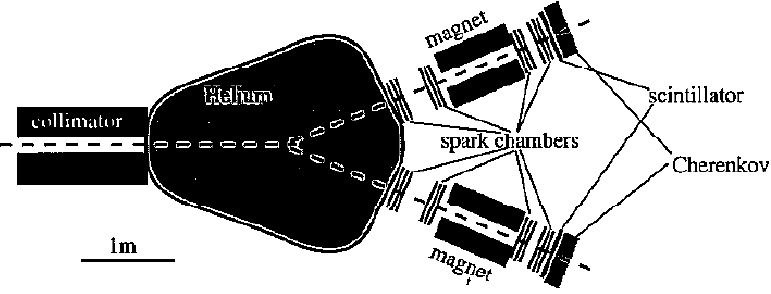
\includegraphics[width=0.7\linewidth]{cp_violation/kaon_verval_exp.png}
    \caption{Onderzoek naar het verval van $K$ mesonen}%
    \label{fig:cp_violation/kaon_verval_exp}
\end{figure}

De binnenkomende $K_L^0$'s vervallen in de helium kamer en worden opgevangen door 2 magneten, één voor $\pi^+$ en één voor $\pi^-$. We verwachten dat dit verval zowel een $\pi^+$, een $\pi^-$ en een $\pi^0$ heeft. Bij het recombineren van de waargenomen $\pi^+$ en $\pi^-$ verwachten we dus niet dat dit volledig overeen komen met de massa van $K_L^0$ (135MeV moet aan $\pi^0$ meegegeven worden). Kijken we nu naar de resultaten in figuur \ref{fig:cp_violation/kaon_verval_exp_res} zien we resultaten die we niet zouden verwachten. Als de massa van de samengestelde pionen buiten de zone van de eigenmassa van $K_L^0$ liggen zijn deze mooi uniform in functie van de hoek waaronder ze van elkaar weg gaan. Dit is niet het geval als hun samengestelde massa gelijk is aan de rustmassa van $K_L^0$. Hier krijgen we een piek voor als ze in elkaars tegengestelde richting vervallen. Dit wil dus zeggen dat $K_L^0$ is vervallen in alleen $\pi^+\pi^-$. Dit toont aan dat de $CP$ wordt geschonden met een branching ratio: $B\left(K_{L}^{0} \rightarrow 2 \pi\right)=2 \times 10^{-3} \neq 0$

\begin{figure}[h]
    \centering
    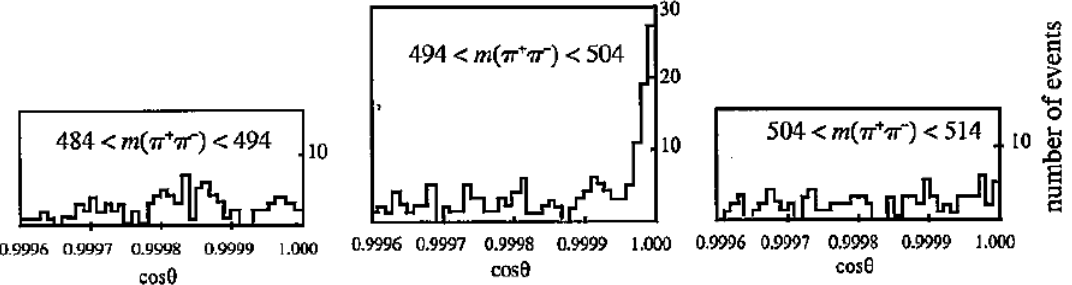
\includegraphics[width=0.8\linewidth]{cp_violation/kaon_verval_exp_res.png}
    \caption{Resulaten van het kaon verval onderzoek}%
    \label{fig:cp_violation/kaon_verval_exp_res}
\end{figure}

\subsection{Mogelijkheden tot $CP$ schending}%
\label{sub:mogelijkheden_tot_cp_schending}

Er zijn verschillende manieren om aan $CP$ schending in het vorige experiment te verklaren.
\begin{itemize}
    \item De $K_S^0$ en $K_L^0$ zijn geen $CP$ eigentoestanden. Dit noemen we de indirecte CP schending.
    \item $CP$ schending in het verval. Het is de interactie verantwoordelijk voor dit verval, de zwakke wisselwerking, schendt $CP$ rechtstreeks. Dit noemen we direct CP verval.
    \item Interferentie met oscillaties. Hier komen we later op terug
\end{itemize}

\subsection{Kaon systeem}%
\label{sub:kaon_systeem}

Onderzoeken we nu deze mogelijke manieren om de $CP$ te schenden op het kaon systeem. Eerst onderzoeken we de indirecte schending. We veronderstellen dat de vrije kaonen $CP$ eigentoestanden zijn en dat $K_S^0\neq K_1^0$ en $K_L^0\neq K_2^0$ zijn. Dit voeren we in door de $CP$ eigentoestanden op te mengen. Bij deze opmengingen wordt er telkens maar een kleine fractie $\epsilon$ van de andere eigentoestand toegevoegd.
\begin{equation}
    \begin{aligned}
        \label{eq:kaon_indirecte_cp_violation_1}
        \left| K_{S}^{0}\right>&=\frac{1}{\sqrt{1+|\epsilon|^{2}}}\left(\left|K_{1}^{0}\right>+\epsilon\left| K_{2}^{0} \right>\right) \\
                               &=\frac{1}{\sqrt{2\left(1+|\epsilon|^{2}\right)}}\left(\left|K^{0}\right>+\left| \bar{K}^{0}\right>+\epsilon\left(\left|K^{0}\right>-\left| \bar{K}^{0}\right>\right)\right) \\
                               &=\frac{1+\epsilon}{\sqrt{2\left(1+|\epsilon|^{2}\right)}}\left|K^{0}\right>+\frac{1-\epsilon}{\sqrt{2\left(1+|\epsilon|^{2}\right)}}\left| \bar{K}^{0}\right>\\
                               &=p_{K}\left|K^{0}\right>+q_{K}\left| \bar{K}^{0}\right>\\
        \left| K_{L}^{0}\right>=& \frac{1}{\sqrt{1+|\epsilon|^{2}}}\left(\epsilon\left|K_{1}^{0}\right>+\left| K_{2}^{0}\right>\right) \\
                                &=p_{K}\left|K^{0}\right>-q_{K}\left| \bar{K}^{0}\right>
    \end{aligned}
\end{equation}
Herschrijven we deze schending nu tot $\eta_{+-}$ en dus in functie van de fase dan vinden we:
\begin{equation}
    \begin{aligned}
        \label{eq:kaon_indirecte_cp_violation_2}
        \eta_{+-} &=\left|\eta_{+-}\right| e^{i \delta_{+-}}=\frac{A\left(K_{L}^{0} \rightarrow \pi^{+} \pi^{-}\right)}{A\left(K_{S}^{0} \rightarrow \pi^{+} \pi^{-}\right)} \\
        \left|\eta_{+-}\right|^{2} &=\frac{\Gamma\left(K_{L}^{0} \rightarrow \pi^{+} \pi^{-}\right)}{\Gamma\left(K_{S}^{0} \rightarrow \pi^{+} \pi^{-}\right)} \\
        \eta_{00} &=\left|\eta_{00}\right| e^{i \delta_{00}}=\frac{A\left(K_{L}^{0} \rightarrow \pi^{0} \pi^{0}\right)}{A\left(K_{S}^{0} \rightarrow \pi^{0} \pi^{0}\right)} \\
        \left|\eta_{00}\right|^{2} &=\frac{\Gamma\left(K_{L}^{0} \rightarrow \pi^{0} \pi^{0}\right)}{\Gamma\left(K_{S}^{0} \rightarrow \pi^{0} \pi^{0}\right)}
    \end{aligned}
\end{equation}
De $A$ refereert hier naar amplitudes die in een ratio herleid kunnen worden tot hun verval breedtes. Voor $\eta_{+-}$ is het verval in  de teller verboden volgens $CP$ en de noemer toegelaten. De $\eta_{00}$ doet hetzelfde maar dan voor het verval naar $\pi^0\pi^0$. Indien $\eta_{+-}=\eta_{00}=\epsilon$ dan hebben we enkel indirecte $CP$ schending. Indien deze $\eta$'s niet gelijk zijn aan elkaar zal er ook directe $CP$ schending voorkomen.\\
{\color{red} Er wordt hier voor deze vergelijkingen niet verwacht dat je ze volledig kan uitwerken en opschrijven. Er wordt wel verwacht dat je het verhaal kan vertellen dat $\eta_{+-}$ overeen komt met de $\pi^+\pi^-$ vervallen en $\eta_{00}$ voor het verval naar $\pi^0\pi^0$. En dat het verschil tussen de 2 uiteindelijk overeen komt met de direct vs indirecte CP schending. Je moet ook kunnen zeggen wat deze 2 soorten CP schending zijn.}\\
In het meest algemene geval krijgen we:
\begin{equation}
    \begin{aligned}
        \label{eq:direct_indirect_algemeen}
        \eta_{+-} &=\epsilon+\epsilon^{\prime} \\
        \eta_{00} &=\epsilon-2 \epsilon^{\prime}
    \end{aligned}
\end{equation}
met $\epsilon$ de indirecte $CP$ schending en $\epsilon'$ de directe. Om het verschil tussen $\epsilon$ en $\epsilon'$ te weten moeten we de $\eta$'s meten.

\subsubsection{Experiment}%
\label{ssub:experiment}

We moeten dus onderzoek doen naar $K^{0} \rightarrow \pi \pi$ met de pion zowel geladen als neutraal. Die zijn vroeger al gedaan maar worden tot de dag van vandaag nog steeds verbetert. We hebben vandaag de dag voor de $\eta$'s de volgende resultaten:
\begin{equation}
    \begin{aligned}
        \label{eq:hedendaagse_eta}
        \left|\eta_{+-}\right| &=(2.232 \pm 0.011) \times 10^{-3} \\
        \left|\eta_{00}\right| &=(2.220 \pm 0.011) \times 10^{-3}
    \end{aligned}
\end{equation}
Om tot deze waarschijnlijkheid te meten is heel veel experimentele ingeniositeit aan te pas moeten komen. Desondanks de vele uren en energie dat hier in gestoken zijn is het niet goed genoeg om te zien of er directe $CP$ schending is. We zijn met deze metingen 100\% zeker dat er $CP$ schending is maar om te zien of we aan directe $CP$ schending doen, moet er met nog hogere precisie gemeten worden. Wat we nu zo precies willen meten is de ratio tussen de $\eta$'s.
\begin{equation}
    \begin{aligned}
        \label{eq:eta_ratio}
        R&=\left|\frac{\eta_{00}}{\eta_{+-}}\right|^{2}\\
         &=\frac{\Gamma\left(K_{L} \rightarrow \pi^{0} \pi^{0}\right)}{\Gamma\left(K_{L} \rightarrow \pi^{+} \pi^{-}\right)} \cdot \frac{\Gamma\left(K_{S} \rightarrow \pi^{+} \pi^{-}\right)}{\Gamma\left(K_{S} \rightarrow \pi^{0} \pi^{0}\right)} \\
         &=\left|\frac{\epsilon-2 \epsilon^{\prime}}{\epsilon+\epsilon^{\prime}}\right|^{2}=\left|\frac{1-2 \epsilon^{\prime} / \epsilon}{1+\epsilon^{\prime} / \epsilon}\right|^{2} \\
         &\approx\left|1-3 \frac{\epsilon^{\prime}}{\epsilon}\right|^{2} \approx 1-3\left(\frac{\epsilon^{\prime}}{\epsilon}+\frac{\epsilon^{\prime *}}{\epsilon^{*}}\right) \\
         &=1-6 \Re\left(\frac{\epsilon^{\prime}}{\epsilon}\right)
    \end{aligned}
\end{equation}
De reden waarom we overstappen naar deze ratio is omdat $\frac{\Gamma\left(K_{L} \rightarrow \pi^{0} \pi^{0}\right)}{\Gamma\left(K_{L} \rightarrow \pi^{+} \pi^{-}\right)}$ en $\frac{\Gamma\left(K_{S} \rightarrow \pi^{+} \pi^{-}\right)}{\Gamma\left(K_{S} \rightarrow \pi^{0} \pi^{0}\right)}$ veel preciser kunnen bepaalt worden dan $\eta_{+-}$ en $\eta_{00}$.\\
Dit is een heel typisch voorbeeld van dubbele ratios die gebruikt worden om veel nauwkeurigere metingen te doen omdat we de tellers en noemers kunnen herschikken in ons voordeel. In dit geval zullen door de herschikte ratios de fluxen van $K_L^0$ en $K_S^0$ wegvallen.\\
Zo was het uiteindelijk mogelijk om deze ratio heel exact te gaan meten.
\begin{equation}
    \begin{aligned}
        \label{eq:eta_ratio_results}
        \left|\frac{\eta_{00}}{\eta_{+-}}\right| &=0.9951 \pm 0.0008(\neq 1) \\
        \Re\left(\frac{\epsilon^{\prime}}{\epsilon}\right) &=(1.65 \pm 0.26) \times 10^{-3} \\
        |\epsilon| &=(2.228 \pm 0.011) \times 10^{-3}
    \end{aligned}
\end{equation}
Het is vandaag de dag dus duidelijk dat er zowel direct als indirecte $CP$ schending zal plaats vinden. M.a.w. is de tijds omkering niet exact. Het vervallen van $K^0$ of het vormen van $K^0$ zal dus niet met exact dezelfde waarschijnlijkheid doorgaan.

\subsection{Materie vs antimaterie}%
\label{sub:materie_vs_antimaterie}

Wat heeft dit nu te maken met materie en antimaterie? Gaan we terug naar de kaon oscilaties. Daar hebben we dat $K^{0} \rightarrow \pi^{-} l^{+} \nu_{l}$ en $\bar{K}^{0} \rightarrow \pi^{+} l^{-} \bar{\nu}_{l}$ wat zuivere leptonische zwakke vervallen zijn. Zoals we gezien hebben in sectie \ref{sub:experiment} is het mogelijk aan de hand van de lading van het lepton om te zien of een $K^0$ of $\bar{K}^0$ is vervallen. Vertrekken we met een zuivere $K^0$ bundel dan zien we enkel positief geladen leptonen en zal $A$ veel groter dan 0 zijn. Na enkele picoseconden zal deze oscilleren in $\bar{K}^0$ en zien we een dal in $A$. Uiteindelijk gaan deze toestanden over naar de $K_L^0$ toestand (alle $K_S^0$ zijn vervallen) die uit even veel $K^0$ als $\bar{K}^0$ bestaat. Voor $t$ groot genoeg moet $A$ dus naar 0 gaan. In de werkelijkheid zien we dat deze niet helemaal naar 0 gaan, er is een kleine asymmetrie. $A$ is iets groter dan 0 wat wil zeggen dat we iets meer positieve leptonen hebben en dus iets meer $K^0$ over hebben. De grafiek dat dit visualiseert is gegeven in figuur \ref{fig:meson_mixing_and_oscillations/kaon_osc_verval}. Het is nu mogelijk om deze asymmetrie uit te schrijven voor de $K_L^0$'s door gebruik te maken van vergelijkingen (\ref{eq:kaon_indirecte_cp_violation_1}).
\begin{equation}
    \begin{aligned}
        \label{eq:asymmetrie_a_l}
        A_{L}=\delta_{L} &=\frac{\Gamma\left(K_{L} \rightarrow \pi^{-} l^{+} \nu\right)-\Gamma\left(K_{L} \rightarrow \pi^{+} l^{-} \bar{\nu}\right)}{\Gamma\left(K_{L} \rightarrow \pi^{-} l^{+} \nu\right)+\Gamma\left(K_{L} \rightarrow \pi^{+} l^{-} \bar{\nu}\right)} \\
                         &=\frac{\left|p_{K}\right|^{2}-\left|q_{K}\right|^{2}}{\left|p_{K}\right|^{2}+\left|q_{K}\right|^{2}} \\
                         &=\frac{|1+\epsilon|^{2}-|1-\epsilon|^{2}}{|1+\epsilon|^{2}+|1-\epsilon|^{2}}=\frac{2 \Re(\epsilon)}{1+|\epsilon|^{2}}
    \end{aligned}
\end{equation}
In deze uitwerking verwaarlozen we de directe $CP$ schending (deze is ook niet waargenomen hier). We zien dus dat dit een effect is van niet meer dan een aantal promille. Het mooie is dat de $\epsilon$ die we hier meten overeen komt bij het onderzoek van het pionisch verval.\\
De experimentele waardes voor de asymmetrie zijn gegeven door $A_{L}=(3.32 \pm 0.06) \times 10^{-3}$. Nu is het mogelijk om een definitie te geven aan materie en antimaterie. Materie wordt gedefinieerd als: Wanneer de lading van de kern gelijk is aan de lading van het meest waarschijnlijke lepton in het $K_L$ verval (positief) is wat wij materie noemen. Dit is contra intuïtief omdat we meer elektronen tegenkomen dan positronen. Bij het ontstaan van het universum zijn de elektronen en positronen hoofdzakelijk niet gemaakt via dit kanaal maar eerder via de neutrinos. Dit zal duidelijker worden in het volgende hoofdstuk.

\subsection{Matrix element van Kaon oscillaties}%
\label{sub:matrix_element}

De vraag is nu of dit consistent is met wat we al hadden. Kijken we hiervoor terug naar de box diagrammen van deze oscillaties en hun matrix elementen.
\begin{minipage}[c]{0.5\textwidth}
    \begin{center}
        \begin{tikzpicture}
            \begin{feynman}
                \vertex (a1) {\(\overline s\)};
                \vertex[right=1cm of a1] (a2);
                \vertex[right=1cm of a2] (a3);
                \vertex[right=1cm of a3] (a4) {\(\overline d\)};

                \vertex[below=1cm of a1] (b1) {\(d\)};
                \vertex[right=1cm of b1] (b2);
                \vertex[right=1cm of b2] (b3);
                \vertex[right=1cm of b3] (b4) {\(s\)};

                \diagram* {
                    (b1) -- [fermion] (b2) -- [fermion, edge label={\(u,c,t\)}] (a2) -- [fermion] (a1),
                    (a4) -- [fermion] (a3) -- [fermion, edge label={\(u,c,t\)}] (b3) -- [fermion] (b4),
                    (a2) -- [boson, edge label=\(W\)] (a3),
                    (b2) -- [boson, edge label=\(W\)] (b3),
                };
                \draw [decoration={brace}, decorate] (b1.south west) -- (a1.north west)
                node [pos=0.5, left] {\(K^{0}\)};
                \draw [decoration={brace}, decorate] (a4.north east) -- (b4.south east)
                node [pos=0.5, right] {\(\bar{K}^{0}\)};
            \end{feynman}
        \end{tikzpicture}
    \end{center}
\end{minipage}\noindent
\begin{minipage}[c]{0.5\textwidth}
    \begin{center}
        \begin{tikzpicture}
            \begin{feynman}
                \vertex (a1) {\(\overline s\)};
                \vertex[right=1cm of a1] (a2);
                \vertex[right=1cm of a2] (a3);
                \vertex[right=1cm of a3] (a4) {\(\overline d\)};

                \vertex[below=1cm of a1] (b1) {\(d\)};
                \vertex[right=1cm of b1] (b2);
                \vertex[right=1cm of b2] (b3);
                \vertex[right=1cm of b3] (b4) {\(s\)};

                \diagram* {
                    (b1) -- [fermion] (b2) -- [fermion, edge label={\(u,c,t\)}] (b3) -- [fermion] (b4),
                    (a1) -- [anti fermion] (a2) -- [anti fermion, edge label={\(\bar{u},\bar{c},\bar{t}\)}] (a3) -- [anti fermion] (a4),
                    (b2) -- [boson, edge label=\(W\)] (a2),
                    (a3) -- [boson, edge label=\(W\)] (b3),
                };
                \draw [decoration={brace}, decorate] (b1.south west) -- (a1.north west)
                node [pos=0.5, left] {\(K^{0}\)};
                \draw [decoration={brace}, decorate] (a4.north east) -- (b4.south east)
                node [pos=0.5, right] {\(\bar{K}^{0}\)};
            \end{feynman}
        \end{tikzpicture}
    \end{center}
\end{minipage}
Bij elke vertex in deze diagrammen zien we dat de CKM-matrix elementen tevoorschijn zullen komen. Zo krijgen we uiteindelijk voor elke mogelijk intermediaire quark een matrix element $\mathcal{M}_{q q^{\prime}} \propto V_{q d} V_{q s}^{*} V_{q^{\prime} s}^{*} V_{q^{\prime} d}$. Het totale matrix element zal dan ongeveer overeen komen met $\mathcal{M} \approx \mathcal{M}_{u u}+\mathcal{M}_{u c}+\mathcal{M}_{c u}+\mathcal{M}_{c c}$. De matrixelementen waar een top quark voorkomt zullen verwaarloosbaar klein zijn vanwege zijn grote massa. We hebben enkel opmenging van de eerste en 2de generatie hier wat wil zeggen dat we kunnen gebruik maken van de Cabbibo hoeken:
\begin{equation}
    \begin{aligned}
        \label{eq:cab_hoeken}
        V_{u d} &\approx V_{c s} \approx \cos \theta_{C} \\
        V_{u s} &\approx-V_{c d} \approx \sin \theta_{C}
    \end{aligned}
\end{equation}
Dit kan dan uitgewerkt worden (zie hiervoor Thompson, dit is niet echt verwacht vanbuiten te kunnen in deze cursus) en krijgen we een massaverschil dat er als volgt uitziet:
\begin{equation}
    \begin{aligned}
        \label{eq:kaon_osc_massaverschil}
        \Delta m \approx \frac{G_{F}^{2}}{3 \pi^{2}} \sin ^{2} \theta_{C} \cos ^{2} \theta_{C} f_{K}^{2} m_{K} \frac{\left(m_{c}^{2}-m_{u}^{2}\right)^{2}}{m_{c}^{2}}
    \end{aligned}
\end{equation}
De $G_F^2$ komt van de koppelingen aan de 2 $W$ bosonen wat een 2de orde zwakke wisselwerking is. De sinus en cosinus termen komen van de CKM-matrix elementen en de massatermen komen van het uitwerken van de matrixelementen. Wat belangrijk is om te in te zien aan deze massatermen, is dat als $m_c$ gelijk zou zijn aan $m_u$ dat er geen massaverschil zou zijn tussen $K^0$ en $\bar{K}^0$. De kaonen zouden nog steeds opmengen met elkaar maar de oscillaties zouden volledig gedempt zijn. Ten laatste hebben we ook nog een $f_K^2$ vorm factor term over om de hadronische kaonen te beschrijven. Dit is niet mogelijk om te doen aan de hand van first principles.\\
Theoretisch uitgerekend komen we uit dat het massaverschil $\Delta m \approx 5 \times 10^{-12}$MeV moet zijn en experimenteel vinden we $3.5 \times 10^{-12}$MeV wat vrij goed overeen komt.\\
{\color{red} Waar is Ryckbosch vooral in geïnteresseerd? Het kunnen uitleggen waarom $G_F^2$, de sinussen en cosinussen... aanwezig zijn. Niet echt in de wiskunde hoe de matrix elementen worden uitgewerkt. Daar is geen tijd voor in een semestervak.}\\

\subsection{$CP$ schending}%
\label{sub:_cp_schending}

Deze uitrekeningen zeggen misschien iets over de oscillaties maar niets over de $CP$ schending. Om dit theoretisch te kunnen bekijken moeten we er de 3de generatie matrix elementen aan toevoegen $\mathcal{M}_{12} \propto V_{q d} V_{q s}^{*} V_{t d} V_{t s}^{*}$. De reden hiervoor is dat het fase element werkt tussen de eerste en 3de fase. Deze faseterm zal dus alleen maar voorkomen in $\mathcal{M}$ als $V_{td}$ daarin zal voorkomen. Bekijken we nu deze matrix elementen als we aan tijd inversie doen.\\
\begin{minipage}[c]{0.5\textwidth}
    \begin{center}
        \begin{tikzpicture}
            \begin{feynman}
                \vertex (a1) {\(\overline s\)};
                \vertex[right=1cm of a1] (a2);
                \vertex[right=1cm of a2] (a3);
                \vertex[right=1cm of a3] (a4) {\(\overline d\)};

                \vertex[below=1cm of a1] (b1) {\(d\)};
                \vertex[right=1cm of b1] (b2);
                \vertex[right=1cm of b2] (b3);
                \vertex[right=1cm of b3] (b4) {\(s\)};

                \diagram* {
                    (b1) -- [fermion] (b2) -- [fermion, edge label={\(u,c,t\)}] (a2) -- [fermion] (a1),
                    (a4) -- [fermion] (a3) -- [fermion, edge label={\(u,c,t\)}] (b3) -- [fermion] (b4),
                    (a2) -- [boson, edge label=\(W\)] (a3),
                    (b2) -- [boson, edge label=\(W\)] (b3),
                };
                \draw [decoration={brace}, decorate] (b1.south west) -- (a1.north west)
                node [pos=0.5, left] {\(K^{0}\)};
                \draw [decoration={brace}, decorate] (a4.north east) -- (b4.south east)
                node [pos=0.5, right] {\(\bar{K}^{0}\)};
            \end{feynman}
        \end{tikzpicture}
    \end{center}
\end{minipage}\noindent
\begin{minipage}[c]{0.5\textwidth}
    \begin{center}
        \begin{tikzpicture}
            \begin{feynman}
                \vertex (a1) {\(\overline d\)};
                \vertex[right=1cm of a1] (a2);
                \vertex[right=1cm of a2] (a3);
                \vertex[right=1cm of a3] (a4) {\(\overline s\)};

                \vertex[below=1cm of a1] (b1) {\(s\)};
                \vertex[right=1cm of b1] (b2);
                \vertex[right=1cm of b2] (b3);
                \vertex[right=1cm of b3] (b4) {\(d\)};

                \diagram* {
                    (b1) -- [anti fermion] (b2) -- [anti fermion, edge label={\(u,c,t\)}] (a2) -- [anti fermion] (a1),
                    (a4) -- [anti fermion] (a3) -- [anti fermion, edge label={\(u,c,t\)}] (b3) -- [anti fermion] (b4),
                    (a2) -- [boson, edge label=\(W\)] (a3),
                    (b2) -- [boson, edge label=\(W\)] (b3),
                };
                \draw [decoration={brace}, decorate] (b1.south west) -- (a1.north west)
                node [pos=0.5, left] {\(\bar{K}^{0}\)};
                \draw [decoration={brace}, decorate] (a4.north east) -- (b4.south east)
                node [pos=0.5, right] {\(K^{0}\)};
            \end{feynman}
        \end{tikzpicture}
    \end{center}
\end{minipage}
\begin{equation}
    \begin{aligned}
        \label{eq:kaon_osc_tijd_inv}
        \mathcal{M}_{12} \propto V_{q d} V_{q s}^{*} V_{t d} V_{t s}^{*} \quad \mathcal{M}_{21} \propto V_{q d}^{*} V_{q s} V_{t d}^{*} V_{t s}=\mathcal{M}_{12}^{*}
    \end{aligned}
\end{equation}
Er zal $CP$ schending plaatsvinden als $\mathcal{M}_{12} \neq \mathcal{M}_{12}^{*}$ is (Dit komt van $CPT$ die behouden moet worden). In de standaard parametrisatie is het alleen mogelijk dat deze afwijken door de imaginaire delen in de koppeling van de eerste met derde generatie $V_{u b}$ en $V_{t d}$.\\
Het is mogelijk om aan te tonen (zie de Thompson) dat de indirecte $CP$ schending wordt gegeven door:
\begin{equation}
    \begin{aligned}
        \label{eq:direct_cp_viol_kaon}
        |\epsilon| \approx \frac{\Im\left(\mathcal{M}_{12}\right)}{\sqrt{2} \Delta m} \quad|\epsilon| \propto \eta(1-\rho+c s t .)
    \end{aligned}
\end{equation}
Uit $\epsilon$ is het dus mogelijk om de faseterm in de CKM-matrix te bepalen. Het probleem hierbij is dat dit moeilijk te bepalen is met de lichte kaonen. We willen het liefst een zwaarder meson bekijken dat een $b$ quark bevat die bijna uitsluitend bindt met de $t$ quark. De perfecte kandidaat hiervoor is het $B$ meson.

\subsection{$B$-systeem}%
\label{sub:_b_systeem}

\begin{center}
    \begin{tikzpicture}
        \begin{feynman}
            \vertex (a1) {\(\overline b\)};
            \vertex[right=1cm of a1] (a2);
            \vertex[right=1cm of a2] (a3) node [above=0.1em of a3] {\(V_{td}^*\)};
            \vertex[right=1cm of a3] (a4) {\(\overline d\)};

            \vertex[below=1cm of a1] (b1) {\(d\)};
            \vertex[right=1cm of b1] (b2) node [below=0.2em of b2] {\(V_{td}\)};
            \vertex[right=1cm of b2] (b3);
            \vertex[right=1cm of b3] (b4) {\(b\)};

            \diagram* {
                (b1) -- [fermion] (b2) -- [fermion, edge label={\(u,c,t\)}] (a2) -- [fermion] (a1),
                (a4) -- [fermion] (a3) -- [fermion, edge label={\(u,c,t\)}] (b3) -- [fermion] (b4),
                (a2) -- [boson, edge label=\(W\)] (a3),
                (b2) -- [boson, edge label=\(W\)] (b3),
            };
            \draw [decoration={brace}, decorate] (b1.south west) -- (a1.north west)
            node [pos=0.5, left] {\(B^{0}\)};
            \draw [decoration={brace}, decorate] (a4.north east) -- (b4.south east)
            node [pos=0.5, right] {\(\bar{B}^{0}\)};
        \end{feynman}
    \end{tikzpicture}
\end{center}
Omdat de bottom quark zo goed als alleen zal koppelen met de top quark hebben we nog maar 1 matrix element over.
\begin{equation}
    \begin{aligned}
        \label{eq:mat_el_b_osc}
        \mathcal{M}_{12} \propto\left(V_{t d} V_{t b}^{*}\right)^{2}
    \end{aligned}
\end{equation}
Zoals voor het Kaon systeem kunnen we hier terug het massaverschil berekenen en zien dat $\Delta m_{d} \propto\left|V_{t d}^{2}\right|$. Het is nu mogelijk om die fase te bekijken $V_{t d}=\left|V_{t d}\right| e^{-i \beta}$. De reden waarom er verschillende notaties worden gebruikt voor de fase is omdat er op dit moment nog veel onderzoek naar wordt gedaan en de benaming nog niet echt vast ligt.\\
Bekijken we nu de opmenging:
\begin{equation}
    \begin{aligned}
        \label{eq:b_opmenging}
        \left| B_{L}\right>&=\frac{1}{\sqrt{2}}\left(\left|B^{0}\right>+e^{-i 2 \beta}\left| \bar{B}^{0}\right>\right) \\
        \left| B_{H}\right>&=\frac{1}{\sqrt{2}}\left(\left|B^{0}\right>-e^{-i 2 \beta}\left| \bar{B}^{0}\right>\right)
    \end{aligned}
\end{equation}
We hebben hier deze fase aan $B_L$ en $B_H$ toegevoegd waardoor de verdeling niet perfect 50-50 meer zal zijn. Deze zal de indirecte $CP$ schending weergeven.\\
Dit onderzoek werd voor het eerst gedaan aan BaBar waar het verval $B^{0}\left(\bar{B}^{0}\right) \rightarrow J / \Psi K_{S}^{0}$ wordt bekeken. Hier zijn we terug geïnteresseerd in de $CP$ van de toestanden.
\begin{equation}
    \begin{aligned}
        \label{eq:cp_toestanden}
        C P\left|J / \Psi\right>&=+\left| J / \Psi\right>\\
        C P\left|K_{S}^{0}\right>&=+\left| K_{S}^{0}\right>\\
        \Rightarrow C P\left(\left| J / \Psi K_{S}^{0}\right>\right)&=-1
    \end{aligned}
\end{equation}
Hoe komen we nu aan de $CP$ van $J / \Psi$? De pariteit hiervan is heel makkelijk. Dit is een vector boson dus $P=-1$ en $S=1$. Voor $C$ moeten we naar de symmetrie van het deeltje kijken.

\begin{table}[h]
    \centering
    \caption{Symmetrie van $J / \Psi$}
    \label{tab:label}
    \begin{tabular}{cccc}
        $\Psi$ & $\Phi(r)$ & $t(s)$ & $\psi(c)$ \\
        $-$    & $+$       & $+$    & $-$
    \end{tabular}
\end{table}

Het radiaal deel is positief wegens in de grondtoestand te zitten en het spin gedeelte is positief wegens een totale spin van 1 te hebben. Omdat de totale golffunctie negatief moet zijn moet Het C pariteit gedeelte negatief zijn. Zo krijgen we dus voor $CP$ positief wordt. Omdat $J$ ook moet behouden zijn en de de spin van alle andere deeltjes dan $J / \Psi$ is 0 en om aan een $J$ van 0 te geraken, moet $L=1$ zijn. Zo krijgen we uiteindelijk $C P\left(\mid J / \Psi K_{S}^{0}>\right)=-1$.\\
Het is nu mogelijk dat $B^{0} \rightarrow J / \Psi K_{S}$ en $B^{0} \rightarrow \bar{B}^{0} \rightarrow J / \Psi K_{S}$ vervallen interfereren met elkaar. Hierdoor worden we gevoelig voor de verschillen tussen $B^{0} \rightarrow \bar{B}^{0}$ en $\bar{B}^{0} \rightarrow B^{0}$.\\
Babar is een asymmetrisch experiment waar een positron en elektron worden omgezet in $B$ mesonen.

\begin{figure}[h]
    \centering
    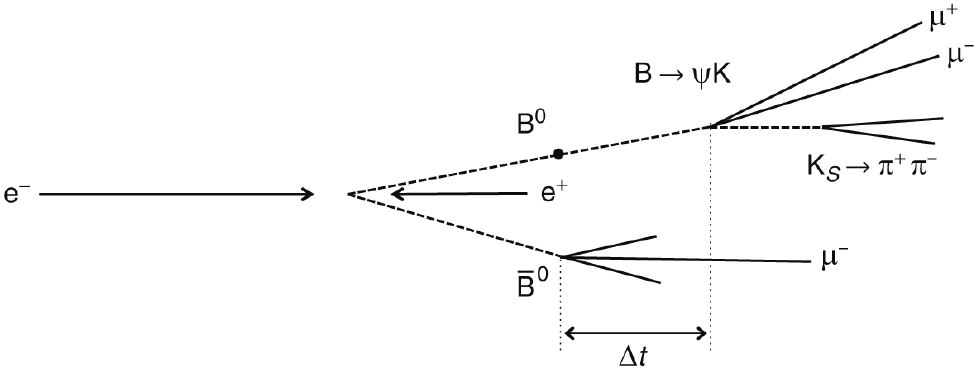
\includegraphics[width=0.6\linewidth]{cp_violation/babar.png}
    \caption{Babar experiment om $CP$ schending te bekijken}%
    \label{fig:cp_violation/babar}
\end{figure}

De lading van de leptonen tonen zoals bij de kaon oscillaties of een $B^0$ en $\bar{B}^0$ vervallen is. Dit gebruiken we natuurlijk om de asymmetrie te onderzoeken. Wat we nu precies willen onderzoeken is het tijdverschil tussen het verval van $\bar{B}^0$ en dat van $B^0$.
\begin{equation}
    \begin{aligned}
        \label{eq:cp_asymmetrie}
        A_{C P}=\frac{\Gamma\left(\bar{B}^{0} \rightarrow J / \Psi K_{S}^{0}\right)-\Gamma\left(B^{0} \rightarrow J / \Psi K_{S}^{0}\right)}{\Gamma\left(\bar{B}^{0} \rightarrow J / \Psi K_{S}^{0}\right)+\Gamma\left(B^{0} \rightarrow J / \Psi K_{S}^{0}\right)}=\sin \left(\Delta m_{d} \cdot \Delta t\right) \sin (2 \beta)
    \end{aligned}
\end{equation}

\begin{figure}[h]
    \centering
    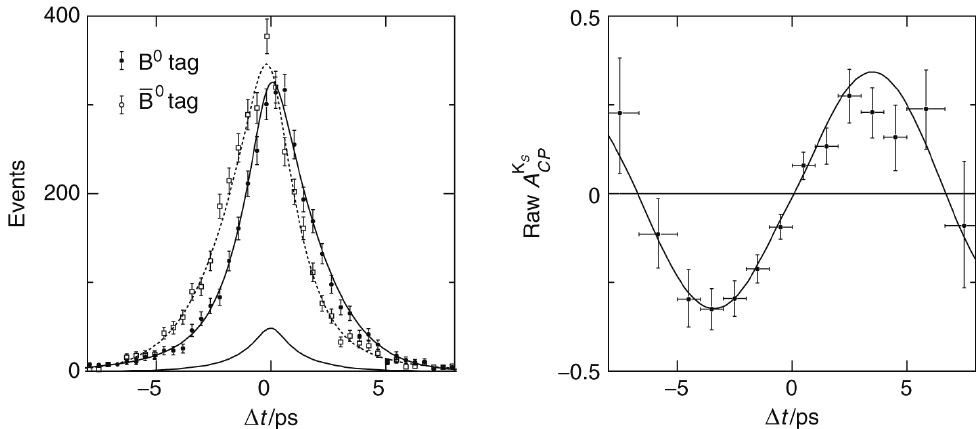
\includegraphics[width=0.6\linewidth]{cp_violation/babar_results.png}
    \caption{Babar resultaten van $CP$ schending}%
    \label{fig:cp_violation/babar_results}
\end{figure}

De reden dat voor grotere negatieve $\Delta t$ geen vervallen zijn is omdat de $B$ mesonen nog niet aangemaakt zijn. Voor be lage waarden voor positieve $\Delta t$ is dat we aan het einde van de detector zijn gekomen en niet meer kunnen meten. Het kleine verschil die je ziet in de curves zullen neerkomen op een mooie oscillatie met frequentie $\Delta m_d \cdot \Delta t$ en amplitude afhankelijk van $\beta$. We vinden uiteindelijk dat $\sin (2 \beta)=0.685 \pm 0.032$ is.

\subsection{Unitaire driehoek}%
\label{sub:unitaire_driehoek}

We hebben al gekeken naar de som van de kwadraten van de rijen en kolommen van de CKM-matrix. We kunnen nu nog een stap verder gaan.
\begin{equation}
    \begin{aligned}
        \label{eq:unitaire_driehoek}
        V^{\dagger} V=\left(\begin{array}{ccc}
                V_{u d}^{*} & V_{c d}^{*} & V_{t d}^{*} \\
                V_{u s}^{*} & V_{c s}^{*} & V_{t s}^{*} \\
                {\color{red} V_{u b}^{*}} & {\color{red} V_{c b}^{*}} & {\color{red} V_{t b}^{*}}
                \end{array}\right)\left(\begin{array}{ccc}
                {\color{red} V_{u d}} & V_{u s} & V_{u b} \\
                {\color{red} V_{c d}} & V_{c s} & V_{c b} \\
                {\color{red} V_{t d}} & V_{t s} & V_{t b}
                \end{array}\right)=\left(\begin{array}{ccc}
                1 & 0 & 0 \\
                0 & 1 & 0 \\
                {\color{red} 0} & 0 & 1
        \end{array}\right)
    \end{aligned}
\end{equation}
De vermenigvuldiging van een rij met de kolom moet natuurlijk ook 0 of 1 zijn als we kijken naar het matrix product.
\begin{equation}
    \begin{aligned}
        \label{eq:matrix_vermenigvuldiging}
        V_{u b}^{*} V_{u d}+V_{c b}^{*} V_{c d}+V_{t b}^{*} V_{t d}=0
    \end{aligned}
\end{equation}
Bekijken we deze vergelijking in het complex vlak dan komt dit overeen met een driehoek.

\begin{figure}[h]
    \centering
    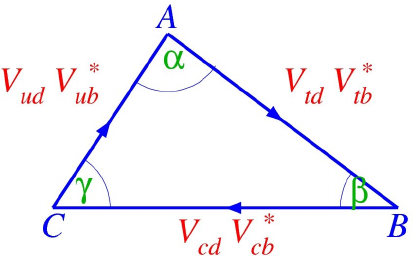
\includegraphics[width=0.6\linewidth]{cp_violation/complexe_driehoek.png}
    \caption{Driehoek voorstelling van matrix vermenigvuldiging}%
    \label{fig:cp_violation/complexe_driehoek}
\end{figure}

De $cd$ en $cb$ componenten is bij constructie reëel en de andere 2 termen hebben een imaginaire component. Het is zo mogelijk om uit te rekenen dat:
\begin{equation}
    \begin{aligned}
        \label{eq:driehoeksvoorstelling_mat_vermenigvuldiging}
        \frac{V_{u b}^{*} V_{u d}}{V_{c b}^{*} V_{c d}} &=(\rho+i \eta)\left(\frac{\lambda^{2}}{2}-1\right) \\
                                                        &=\bar{\rho}+i \bar{\eta}
    \end{aligned}
\end{equation}
Zo bekomen we dat de coördinaten van deze driehoek gegeven worden door $C=(0,0)$, $B=(1,0)$ en $A=(\bar{\rho}, \bar{\eta})$.\\
Dit kan nu op meerdere manieren gemeten worden:
\begin{itemize}
    \item $CA$ zijde: $V_{u b}^{*}=A \lambda^{3}(\rho+i \eta)$ Al deze componenten hiervan hebben we al experimenteel bepaald. $V_{ud}$ is reëel en is zeer goed gekend.
    \item $AB$ zijde: $V_{t d}=A \lambda^{3}(1-\rho-i \eta)$ samen met $V_{t d}=\left|V_{t d}\right| e^{-i \beta}$ is het mogelijk om in te zien dat $\tan \beta=\frac{\eta}{1-\rho}$.
\end{itemize}
We willen dus eigenlijk de coördinaten van $A$ bepalen. Dit kunnen we doen op verschillende manieren die we samenvoegen in 1 plot (figuur \ref{fig:cp_violation/driehoek_a_bepalen}).

\begin{figure}[ht]
    \centering
    \subfloat[2012]{
        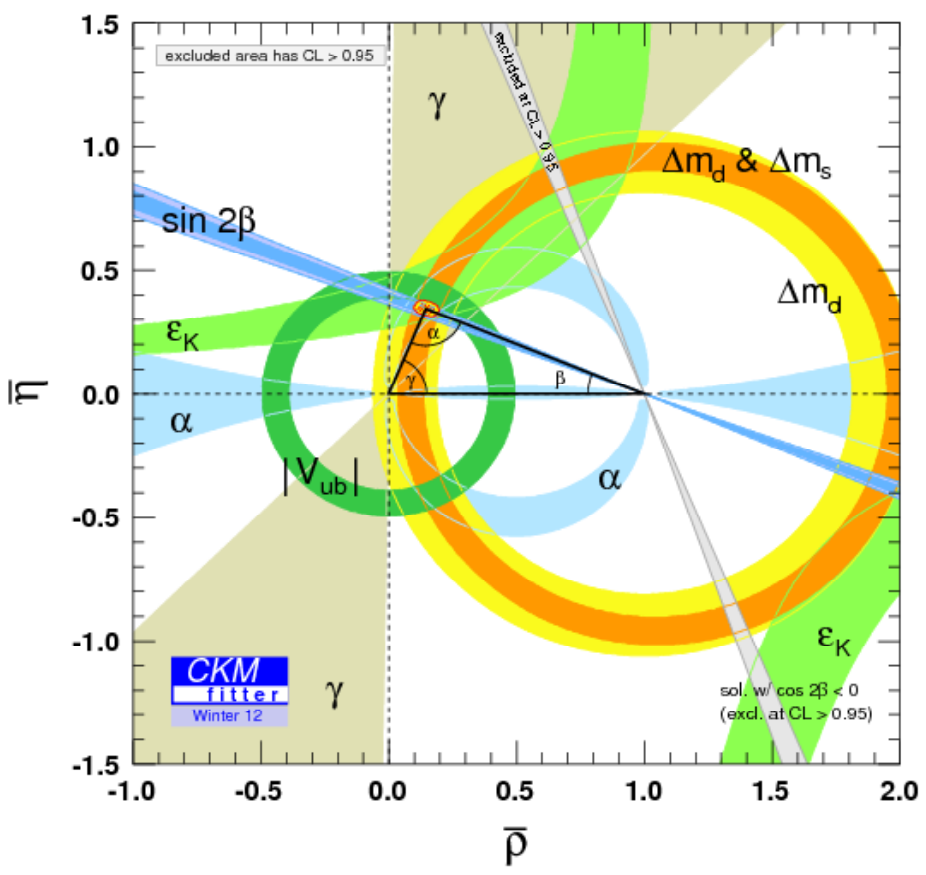
\includegraphics[width=0.4\textwidth]{cp_violation/driehoek_a_bepalen_12.png}
        \label{fig:cp_violation/driehoek_a_bepalen_12}
    }
    \hfill
    \subfloat[2018]{
        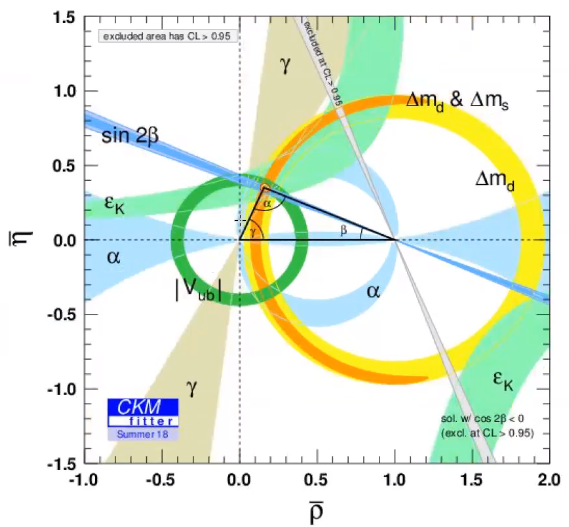
\includegraphics[width=0.4\textwidth]{cp_violation/driehoek_a_bepalen_18.png}
        \label{fig:cp_violation/driehoek_a_bepalen_18}
    }\\
    \subfloat[2018 zoom]{
        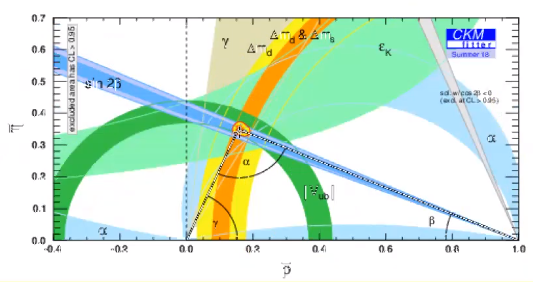
\includegraphics[width=0.6\textwidth]{cp_violation/driehoek_a_bepalen_zoom.png}
        \label{fig:cp_violation/driehoek_a_bepalen_zoom}
    }
    \caption{Alle metingen samengevoegd om $A$ te bepalen}%
    \label{fig:cp_violation/driehoek_a_bepalen}
\end{figure}

De zijde $CA$ kon  gehaald worden uit $|V_{ub}|$ en de zijde $AB$ door $|V_{td}|$ en $|V_{tb}|$ of specifiek de metingen van $\Delta m_d$ (oscillatie $B^0/\bar{B}^0$ systeem) en $\Delta m_s$ (oscillatie $B_S/\bar{B}_S$ systeem). Deze metingen zijn enkel gevoelig voor de som van de reële en imaginaire delen. Om nu enkel het imaginaire gedeelte te bepalen moeten we bijvoorbeeld kijken naar de $CP$ schending in het kaon systeem $\varepsilon_K$ of $CP$ schending in het $B$ systeem krijgen we $\sin 2\beta$. We zien uiteindelijk dat er maar een klein gebied is waar overlap tussen al deze metingen mogelijk is. We kunnen hieruit afleiden dat alle metingen die we gedaan hebben consistent zijn met een overeenkomstig punt in $(\rho, \eta)$. De CKM-matrix is dus unitair.\\
Dit betekent dat alle indirecte $CP$ schending die we waarnemen dat deze consistent is. Zo begrijpen we ook dat er juist 3 generaties zijn in het heelal die we in essentie niet zouden moeten hebben om een werkend heelal te beschrijven. Kijken we nu nog eens terug naar de Wolfenstein representatie van de CKM-matrix, zien we dat we alle parameters hebben bepaald.
\begin{equation}
    \begin{aligned}
        \label{eq:wolfenstein_ckm_revisit}
        V_{C K M}&=\left(\begin{array}{ccc}
                1-\lambda^{2} / 2 & \lambda & A \lambda^{3}(\rho-i \eta) \\
                -\lambda & 1-\lambda^{2} / 2 & A \lambda^{2} \\
                A \lambda^{3}(1-\rho-i \eta) & -A \lambda^{2} & 1
        \end{array}\right)+O\left(\lambda^{4}\right)\\
        \lambda &=0.2253 \pm 0.0007 \\
        A &=0.811_{-0.012}^{+0.022} \\
        \rho &=0.13 \pm 0.02 \\
        \eta &=0.345 \pm 0.014
    \end{aligned}
\end{equation}

\subsection{Conclusies $CP$ schending}%
\label{sub:conclusies_cp_schending}

Wat hebben we nu allemaal geleerd van de oscillaties?
\begin{itemize}
    \item Deeltjes worden vaak als flavour eigentoestanden gecreëerd via de sterke wisselwerking.
    \item Deze deeltjes propageren als fysische massa eigentoestanden
    \item Uiteindelijk vervallen ze als ofwel flavour toestanden of $CP$ eigentoestanden, afhankelijk van wat de eindtoestand is.
\end{itemize}
Over de $CP$ schending hebben we geleerd dat:
\begin{itemize}
    \item De $CP$ schending komt van de complexe fase in de CKM-matrix.
    \item We hebben dit zowel in het $K^0$ als $B^0$ systemen waargenomen. We zouden dit ook graag zien in $D$ systemen maar daar zijn we nog maar juist in staat om de oscillaties waar te nemen.
    \item Alle metingen die we doen zijn consistent met 1 complexe fase.
\end{itemize}
Hier is nog niet alles mee opgelost. De $CP$ schending die we hier waarnemen is te klein om de $CP$ schending in het universum te verklaren. We moeten hier natuurlijk opletten wat we zeggen. De $CP$ schending in het kaon systeem en deze van het universum zijn niet dezelfde grootheden. De $CP$ schending van $10^{-10}$ van het universum komt van het verschil in aantal baryonen en fotonen in het universum. Deze fotonen komen uiteindelijk van baryon-antibaryon (lepton-antilepton) annihilatie. Indien er geen $CP$ schending zou zijn moeten alle baryonen en antibaryonen annihileren in elkaar in fotonen. Wat we vandaag de dag zien is dat er zo goed als $10^{10}$ keer meer fotonen hebben dan baryonen m.a.w. moet er in de vroege fase van het heelal een heel klein onevenwicht geweest zijn tussen baryonen en antibaryonen van de orde $10^{-10}$ zodat we vandaag de dag nog een kleine overmaat aan baryonen waarnemen die niet geanihileerd zijn. In deze $CP$ schending (meson oscillaties) komt de baryon schending totaal niet aan te pas. Die moet er nog bovenop geplaatst worden. Dit zit niet echt verwerkt in het Standaard Model. Om dit uit te rekenen moet je aan niet pertubatieve QCD doen wat buiten de scope van deze cursus is. Indien je dit zou doorwerken zien we dat we met de faseterm in de CKM-matrix niet toekomen om het heelal te beschrijven. Hetzelfde probleem van de baryonen hebben we ook bij de leptonen wat we in het volgende hoofstuk bekijken.

\end{document}
